\documentclass[12 pt]{article}
\usepackage[utf8]{inputenc}
\usepackage{matlab-prettifier}
\usepackage[portuguese]{babel}
\usepackage{indentfirst}
\usepackage{graphicx}
\usepackage{float}
\usepackage{subcaption}
\usepackage[font=small,labelfont=bf]{caption}
\definecolor{mygreen}{RGB}{28,172,0} % color values Red, Green, Blue
\definecolor{myyellow}{rgb}{1.0, 1.0, 0.8}
\usepackage{mathtools}
\usepackage{multirow}
\usepackage{comment}
\usepackage{xcolor}
\usepackage{colortbl}
\usepackage[normalem]{ulem}               % to striketrhourhg text
\usepackage{amsmath}
\usepackage{amsfonts}
\usepackage{hyperref}
\usepackage{booktabs}
\newcommand\redout{\bgroup\markoverwith
{\textcolor{red}{\rule[0.5ex]{2pt}{0.8pt}}}\ULon}
\renewcommand{\lstlistingname}{Código}% Listing -> Algorithm
\renewcommand{\lstlistlistingname}{Lista de \lstlistingname s}% List of Listings -> List of Algorithms
\usepackage{enumitem}
\usepackage[top=3cm,left=2cm,bottom=2cm, right=2cm]{geometry}

% Configuração para destacar a sintaxe do Python
\lstset{ 
    language=Python,                     % A linguagem do código
    backgroundcolor=\color{myyellow}, % A cor do fundo 
    basicstyle=\ttfamily\footnotesize,   % O estilo do texto básico
    keywordstyle=\color{blue},           % Cor das palavras-chave
    stringstyle=\color{red},             % Cor das strings
    commentstyle=\color{mygreen},          % Cor dos comentários
    numbers=left,                        % Números das linhas à esquerda
    numberstyle=\tiny\color{gray},       % Estilo dos números das linhas
    stepnumber=1,                        % Número de linhas entre os números das linhas
    frame=single,                        % Moldura ao redor do código
    breaklines=true,                     % Quebra automática das linhas longas
    captionpos=t,                        % Posição da legenda
    showstringspaces=false               % Não mostra espaços em branco nas strings
    extendedchars=true,
    literate={º}{{${ }^{\underline{o}}$}}1 {á}{{\'a}}1 {à}{{\`a}}1 {ã}{{\~a}}1 {é}{{\'e}}1 {É}{{\'E}}1 {ê}{{\^e}}1 {ë}{{\"e}}1 {í}{{\'i}}1 {ç}{{\c{c}}}1 {Ç}{{\c{C}}}1 {õ}{{\~o}}1 {ó}{{\'o}}1 {ô}{{\^o}}1 {ú}{{\'u}}1 {â}{{\^a}}1 {~}{{$\sim$}}1
}


\title{%
\textbf{\huge Universidade Federal do Rio de Janeiro} \par
\textbf{\LARGE Instituto Alberto Luiz Coimbra de Pós-Graduação e Pesquisa de Engenharia} \par

\includegraphics[width=8cm]{COPPE UFRJ.png} \par

\textbf{Departamento de Engenharia Elétrica} \par
COE782 - Introdução ao Aprendizado de Máquina \par
Prof. Dr. Markus Vinícius Santos Lima \par 

\vspace{1\baselineskip}
\textit{Lista 3 de exercícios}
}

\author{Luiz Henrique Souza Caldas\\email: lhscaldas@cos.ufrj.br}

\date{\today}

\begin{document}
\maketitle

\newpage

\section{Exercício 1}

Considere o experimento computacional denominado “Polynomial Curve Fitting”, usado
diversas vezes no livro texto (veja páginas 4 e 5 do livro, bem como Apêndice A), considerando a
ordem do modelo sendo M = 9 e o tamanho da amostra sendo N = 10.
Faça:

\begin{enumerate}[label=(\alph*)]
    \item Calcule a solução de mínimos quadrados (LS) \( \mathbf{w_{LS}} \);
    \item Calcule a solução via regressão ridge (escolha um fator de regularização razoável) \( \mathbf{w_{ridge}} \);
    \item Calcule a solução via regressão lasso (escolha um fator de regularização razoável) \( \mathbf{w_{lasso}} \);
    \item Monte uma tabela exibindo os 10 coeficientes \( \mathbf{w} \) para as 3 soluções obtidas nos itens acima e comente/compare os resultados;
    \item Plote uma figura contendo o processo gerador em verde (a senoide), e suas estimativas \( y_{LS} \), \( y_{ridge} \), e \( y_{lasso} \) em preto, azul e vermelho, respectivamente;
    \item Repita todos os itens anteriores para \( N=20 \) e \( N=50 \).
\end{enumerate}

\subsection{Resposta do item (a)}
Para responder esse item foi utilizada a classe $LinearRegression()$ da biblioteca \textit{sklearn} para linguagem \textit{Python}, que realiza uma regressão linear utilizando mínimos quadrados. Foi escolhido um polinômio de ordem 9 como modelo.
\begin{figure}[H]
    \centering
    \caption{Solução para mínimos quadrados (LS)}
    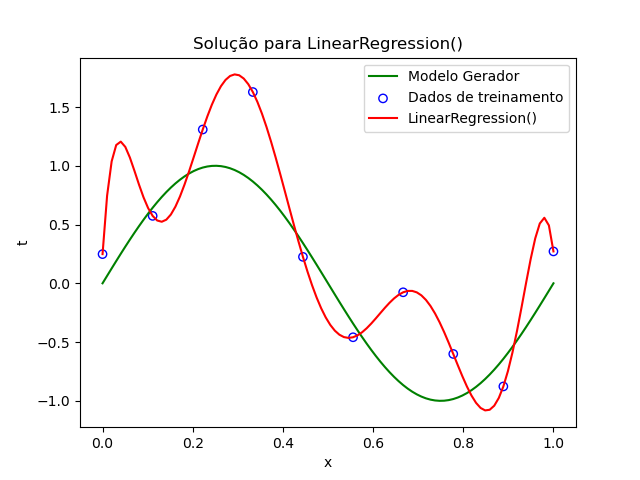
\includegraphics[width=12cm]{E1_a.png}
\end{figure}
A regressão linear por mínimos quadrados não introduz nenhuma regularização e por isso a curva vermelha passa exatamente pelos dados de treinamento, mostrando que eles foram decorados overfitting.


\subsection{Resposta do item (b)}
Para responder esse item foi utilizada a classe $Ridge()$ da biblioteca \textit{sklearn} para linguagem \textit{Python}, que realiza uma regressão linear utilizando mínimos quadrados e regularização de norma $L_2$ (Ridge). Foi escolhido um polinômio de ordem 9 como modelo e o fator de regularização $\lambda$, que na classe $Ridge()$ é chamado de \textit{alpha}, que melhor adaptou a curva ao modelo gerador foi $1^{-0.5}$.
\begin{figure}[H]
    \centering
    \caption{Solução para Ridge com $\lambda = 1^{-0.5}$}
    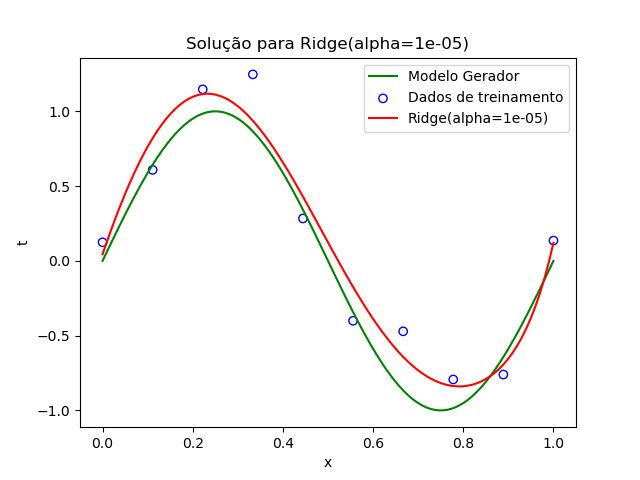
\includegraphics[width=12cm]{E1_b.png}
\end{figure}
A regressão Ridge introduz uma penalização nos coeficientes através do fator de regularização, ajudando a evitar overfitting.

\subsection{Resposta do item (c)}
Para responder esse item foi utilizada a classe $Lasso()$ da biblioteca \textit{sklearn} para linguagem \textit{Python}, que realiza uma regressão linear utilizando mínimos quadrados e regularização de norma $L_1$ (Lasso). Foi escolhido um polinômio de ordem 9 como modelo e o fator de regularização $\lambda$, que na classe $Lasso()$ é chamado de \textit{alpha}, que melhor adaptou a curva ao modelo gerador foi $1^{-0.5}$.
\begin{figure}[H]
    \centering
    \caption{Solução para Lasso com $\lambda = 10^{-0.6}$}
    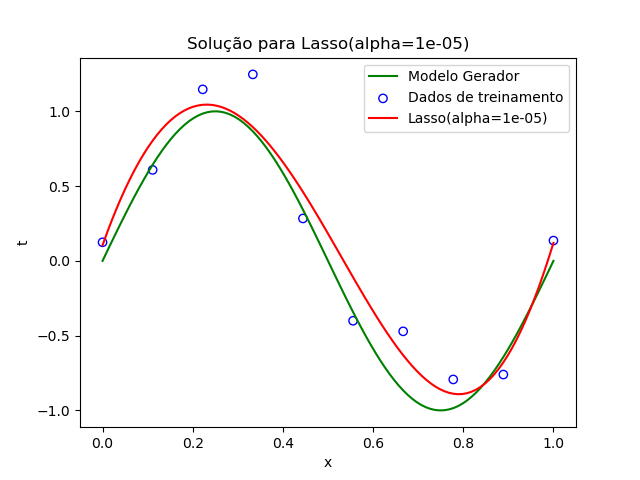
\includegraphics[width=12cm]{E1_c.png}
\end{figure}
A regressão Lasso, assim como a Ridge, introduz uma penalização nos coeficientes através do fator de regularização, ajudando a evitar overfitting.

\subsection{Resposta do item (d)}

A tabela abaixo exibindo os coeficientes para as três soluções permite comparar diretamente o impacto da regularização nos coeficientes.

\begin{table}[H]
\caption{Coeficientes para $N=10$}
\resizebox{\textwidth}{!}{
    \begin{tabular}{lllllllllll}
        \toprule
        Modelo & w0 & w1 & w2 & w3 & w4 & w5 & w6 & w7 & w8 & w9 \\
        \midrule
        LS & 0.00 & 61.35 & -1305.40 & 10864.20 & -43958.49 & 96013.73 & -116795.02 & 75859.90 & -22104.00 & 1363.74 \\
        Ridge & 0.00 & 5.58 & -10.39 & -3.32 & 2.25 & 3.46 & 2.37 & 0.81 & -0.28 & -0.58 \\
        Lasso & 0.00 & 7.87 & -18.23 & 2.99 & 5.02 & 2.16 & 0.11 & 0.00 & -0.00 & 0.09 \\
        \bottomrule
    \end{tabular}
}
\end{table}

A regressão por mínimos quadrados sem regularização tende a produzir coeficientes maiores, um dos sinais que indicam overfitting ou pelo menos uma alta sensibilidade aos dados de treinamento. Enquanto que os coeficientes produzidos pela Ridge e pela Lasso são menores.

Além disso, é possível observar a presença de alguns coeficientes praticamente nulos para a Lasso. Esse resultado era esperado, uma vez que a Lasso, por utilizar a norma $L_1$, tende a produzir uma solução mais esparsa, selecionando atributos mais importantes.

Enquanto isso, a regressão Ridge, apesar de não selecionar atributos como a Lasso, tende a penalizar ainda mais os coeficientes grandes, consequentemente fazendo com que os maiores coeficientes fiquem menores que os produzidos pela Lasso.



\subsection{Resposta do item (e)}
\begin{figure}[H]
    \centering
    \caption{Comparação entre as soluções para $N=10$}
    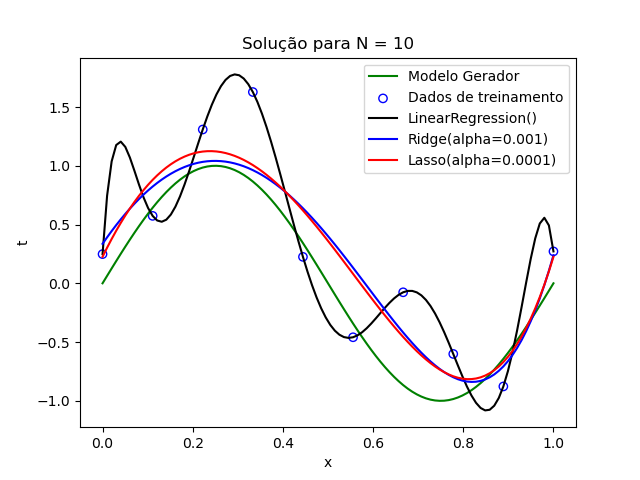
\includegraphics[width=12cm]{E1_e.png}
\end{figure}

\subsection{Resposta do item (f)}

\begin{figure}[H]
    \centering
    \caption{Comparação entre as soluções para $N=20$}
    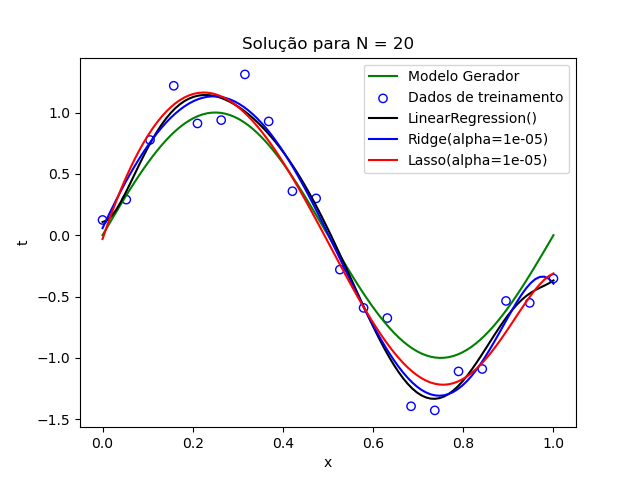
\includegraphics[width=12cm]{E1_f20.png}
\end{figure}
\begin{table}[H]
    \caption{Coeficientes para $N=20$}
    \resizebox{\textwidth}{!}{
        \begin{tabular}{lllllllllll}
            \toprule
            Modelo & w0 & w1 & w2 & w3 & w4 & w5 & w6 & w7 & w8 & w9 \\
            \midrule
            LS & 0.00 & -6.01 & 266.50 & -2042.90 & 7178.62 & -13245.77 & 11993.84 & -3017.56 & -2424.09 & 1296.42 \\
            Ridge & 0.00 & 8.39 & -16.21 & -8.40 & 2.98 & 9.30 & 9.76 & 5.62 & -1.60 & -10.66 \\
            Lasso & 0.00 & 12.42 & -29.59 & 0.72 & 10.39 & 8.98 & 4.55 & 0.00 & -1.36 & -6.72 \\
            \bottomrule
        \end{tabular}
    }
\end{table}

\begin{figure}[H]
    \centering
    \caption{Comparação entre as soluções para $N=50$}
    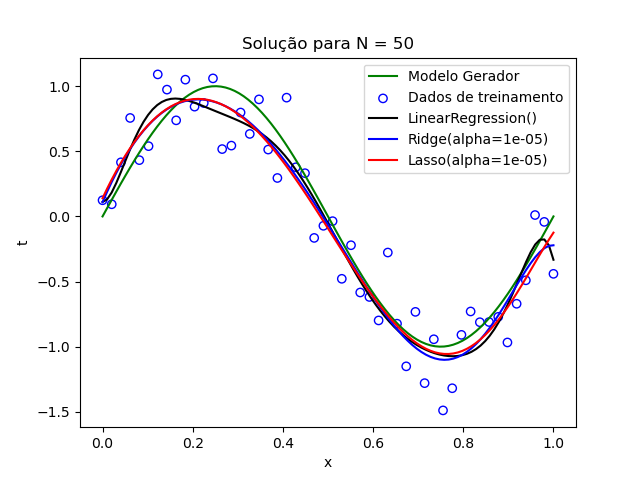
\includegraphics[width=12cm]{E1_f50.png}
\end{figure}
\begin{table}[H]
    \caption{Coeficientes para $N=50$}
    \resizebox{\textwidth}{!}{
        \begin{tabular}{lllllllllll}
            \toprule
            Modelo & w0 & w1 & w2 & w3 & w4 & w5 & w6 & w7 & w8 & w9 \\
            \midrule
            LS & 0.00 & -6.39 & 455.99 & -5270.52 & 27669.17 & -80097.05 & 135776.46 & -134351.92 & 71926.94 & -16103.56 \\
            Ridge & 0.00 & 4.21 & -10.54 & -3.23 & 1.84 & 4.62 & 5.21 & 3.53 & -0.31 & -6.02 \\
            Lasso & 0.00 & 5.12 & -14.48 & 0.36 & 4.73 & 4.19 & 2.22 & 0.00 & -0.00 & -2.74 \\
            \bottomrule
        \end{tabular}
    }
\end{table}

Pelas figuras, podemos observar que a solução para mínimos quadrados começa a sofrer menos com o overfitting à medida que o tamanho da amostra aumenta. Isso se deve ao fato de que o ruído nos dados de treinamento possui uma distribuição gaussiana com média zero. Pela lei dos grandes números, quanto maior a quantidade de dados de treinamento, mais a média da amostra se aproxima da média da distribuição original, que é zero, reduzindo assim o efeito do ruído.

Consequentemente, com mais dados, a solução de mínimos quadrados consegue capturar melhor o padrão subjacente dos dados, e o impacto do ruído diminui. Esse comportamento explica por que a solução de mínimos quadrados apresenta um ajuste mais estável e menos propenso ao overfitting quando o tamanho da amostra aumenta.

No entanto, é importante notar que, mesmo com um aumento no tamanho da amostra, métodos de regularização como a regressão ridge e lasso continuam a fornecer soluções mais robustas e generalizáveis, especialmente em situações onde o ruído pode não ser perfeitamente gaussiano ou quando a complexidade do modelo ainda é alta em relação ao tamanho da amostra.







\section{Exercício 2}

Data Source:
\begin{itemize}
    \item (info) \url{https://web.stanford.edu/~hastie/ElemStatLearn/datasets/prostate.info.txt}
    \item (database) \url{https://web.stanford.edu/~hastie/ElemStatLearn/datasets/prostate.data}
\end{itemize}

“The data for this example come from a study by Stamey et al. (1989). They examined the correlation between the level of prostate-specific antigen (lpsa) and a number of clinical measures in men who were about to receive a radical prostatectomy. The variables are log cancer volume (lcavol), log prostate weight (lweight), age, log of the amount of benign prostatic hyperplasia (lbph), seminal vesicle invasion (svi), log of capsular penetration (lcp), Gleason score (gleason), and percent of Gleason scores 4 or 5 (pgg45).”

Considere a variável (lpsa) como 'target' e as variáveis (lcavol), (lweight), (age), (lbph), (svi), (lcp), (gleason) e (pgg45) como 'entradas'. Siga o roteiro abaixo:
\begin{enumerate}[label=(\alph*)]
    \item Padronize os atributos de entrada para que eles tenham média 0 e variância 1;
    \item Divida o dataset em dois conjuntos, treinamento e teste, conforme indicado nos índices da última coluna (T = treinamento, F = teste);
    \item Encontre o modelo linear de regressão ótimo no critério de mínimos quadrados (solução LS);
    \item Implemente modelos lineares regularizados pelos métodos 'Ridge' e 'Lasso' que minimizam a função objetivo \( L(w) = \frac{1}{2N} RSS(w) + \lambda ||w||^q \). Apresente resultados para \( \lambda = 0.25 \);
    \item Aplicando as regressões 'Ridge' e 'Lasso' e utilizando k-fold cross-validation, é possível selecionar um valor para \( \lambda \) que resulta em um modelo com melhor capacidade de generalização. Isso é feito selecionando o \( \lambda \) relativo à menor estimativa do erro de predição quadrático médio (usualmente chamado de validation score) ao longo dos k-folds. Também é possível selecionar um valor de \( \lambda \) que seleciona o modelo mais simples dentro de uma tolerância da estimativa do erro de predição quadrático médio. Isso é particularmente útil quando se deseja encontrar soluções esparsas (no caso do Lasso) ou de menor norma L2 (no caso do Ridge). Para tal, um critério comumente adotado é a 'Regra de 1 desvio padrão', onde escolhe-se o maior \( \lambda \) cujo validation score seja igual ou pouco menor do que o 'score mínimo' + '1 desvio padrão do score mínimo'.
    \begin{itemize}[label=-]
        \item Monte as curvas de validation score de k-fold cross-validation em função de \( \lambda \) para os modelos regularizados por 'ridge' e 'lasso' (Sugestão: use k = 10, e procure \( \lambda \) em um intervalo [0, 0.5]);
        \item Calcule o desvio padrão do 'score' mínimo em cada respectiva curva e desenhe-o como barra de erro em torno daquele ponto;
        \item Determine o \( \lambda \) que resulta no modelo mais simples de acordo com a 'Regra de 1 desvio padrão';
        \item Treine o modelo final 'ridge' e 'lasso' utilizando todos os dados (de treinamento) e o respectivo \( \lambda \) encontrado e apresente os resultados;
    \end{itemize}
    \item Utilizando o conjunto de teste construído no item (b), calcule a estimativa do erro de predição quadrático médio do conjunto de teste para cada modelo (mínimos quadrados, 'ridge' e 'lasso'). Disserte sobre os resultados obtidos.
    \item (Bônus) Estime o desvio padrão dos coeficientes do modelo obtido pelo método de bootstrap dos resíduos;
\end{enumerate}

Dica: Veja os slides 9 e 10 de \url{http://www.est.ufmg.br/~cristianocs/MetComput/Aula8.pdf}

\subsection{Resposta do item (a)}
Para padronizar os dados de entrada com média zero e variância um, foram selecionadas as colunas 'lcavol', 'lweight', 'age', 'lbph', 'svi', 'lcp', 'gleason' e 'pgg45' como features e depois utilizada a classe $StandardScaler$ da biblioteca  \textit{sklearn} para \textit{python}, que realiza a padronização dos dados pelo método \textit{z-score}.

\subsection{Resposta do item (b)}
O dataset foi dividido utilizando a última coluna (T = treinamento, F = teste), como pedido no enunciado.

\subsection{Resposta do item (c)}
Para implementar o método dos mínimos quadrados foi utilizada a classe $LinearRegression$ da biblioteca  \textit{sklearn} para \textit{python}.
Pelo critério de mínimos quadrados (LS) foram obtidos os seguintes resultados ao se calcular o erro quadrático médio (MSE):

\begin{itemize}
    \item MSE - Treinamento (LS): 0.4391997680583344
    \item  MSE - Teste (LS): 0.5212740055076001
\end{itemize}

O modelo de mínimos quadrados (LS) foi ajustado e apresentou um erro quadrático médio (MSE) de 0.4392 no conjunto de treinamento e 0.5213 no conjunto de teste. A diferença entre os MSE sugere que o modelo tem uma boa capacidade de generalização, mas há espaço para melhoria, possivelmente através de regularização.


\subsection{Resposta do item (d)}
Para implementar o método dos mínimos quadrados foram utilizadas as classe $Ridge$ e $Lasso$ da biblioteca \textit{sklearn} para \textit{python}, ambos utilizando $\lambda=0.25$.
Foram obtidos os seguintes reesultados para cada método ao se calcular o erro quadrático médio:

\begin{itemize}
    \item MSE - Treinamento (Ridge): 0.4392308191154076
    \item MSE - Teste (Ridge): 0.5189192261819305
    \item MSE - Treinamento (Lasso): 0.6207140544187021
    \item MSE - Teste (Lasso): 0.5031909828714028
\end{itemize}

O Ridge apresentou MSE de 0.4392 (treinamento) e 0.5189 (teste), enquanto o Lasso apresentou MSE de 0.6207 (treinamento) e 0.5032 (teste). Os resultados indicam que o Lasso, apesar de ter um MSE de treinamento mais alto, generaliza melhor para o conjunto de teste do que o Ridge para este valor de $\lambda$.

\subsection{Resposta do item (e)}
Para implementar o k-fold cross-validation foi utilizada a classe $KFold$ e o método $cross_val_score$ da biblioteca \textit{sklearn} para \textit{python}, utilizando $k=10$.
As curvas abaixo mostram os resultados para os dois métodos:

\begin{figure}[H]
    \centering
    \caption{Seleção do $\lambda$ para o Ridge}
    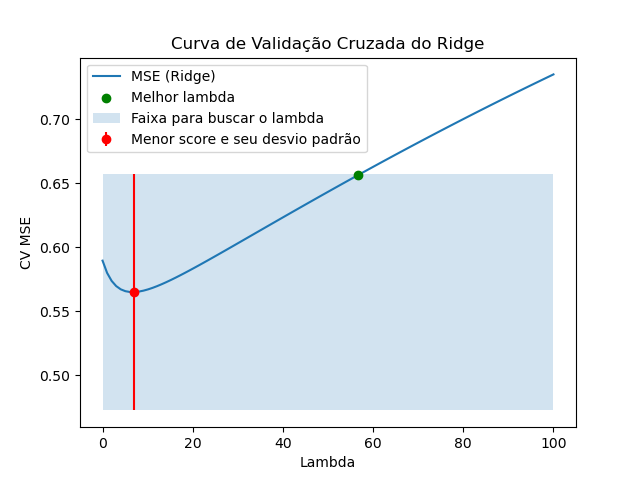
\includegraphics[width=12cm]{ridge.png}
\end{figure}

\begin{itemize}
    \item Melhor lambda (Ridge):  56.56570000000001
\end{itemize}

\begin{figure}[H]
    \centering
    \caption{Seleção do $\lambda$ para o Lasso}
    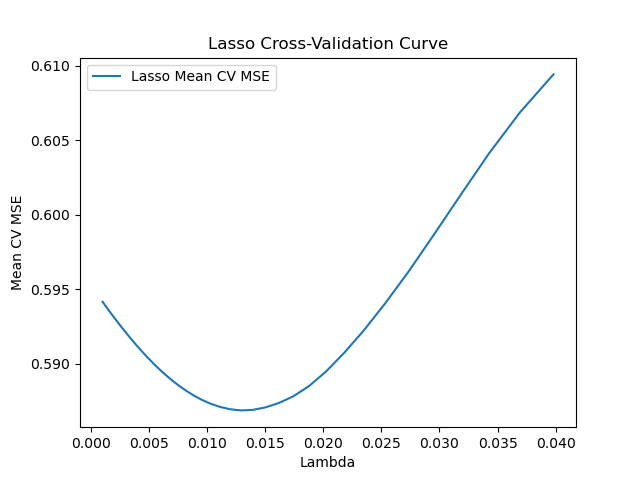
\includegraphics[width=12cm]{lasso.png}
\end{figure}

\begin{itemize}
    \item Melhor lambda (Lasso): 0.17178282828282826
\end{itemize}

O melhor $\lambda$ para Ridge foi 56.5657 e para Lasso foi 0.1718. Isso mostra a importância da validação cruzada para selecionar o hiperparâmetro $\lambda$, que controla o grau de regularização, melhorando a capacidade de generalização dos modelos.

\subsection{Resposta do item (f)}
Utilizando os valores de $\lambda$ obtidos no item (e) para treinar os modelos e avaliando eles no conjunto de teste, foram obtidos os seguintes resultados:

\begin{itemize}
    \item MSE - Teste (Final Ridge): 0.5168573674734896
    \item MSE - Teste (Final Lasso): 0.46269599870385136
\end{itemize}

Os modelos Ridge e Lasso ajustados com os melhores valores de $\lambda$ apresentaram MSE no conjunto de teste de 0.5169 e 0.4627, respectivamente. O Lasso, com $\lambda$ selecionado pela validação cruzada, teve o menor MSE no conjunto de teste, indicando melhor performance de generalização e sugerindo que ele é mais adequado para este problema específico, o que pode ser explicado pela capacidade do Lasso de realizar a seleção de atributos, na qual ele zera o peso de atributos considerados menos importantes durante o treinamento do modelo.

\subsection{Resposta do item (g) (bônus)}
Estimando-se o desvio padrão dos modelos utilizando o método de bootstrap, como explicado no slide fornecido, foram obtidos os seguintes resultados:

\begin{table}[H]
    \caption{Desvio padrão dos coeficientes estimado pelo método de bootstrap}
    \centering
        \begin{tabular}{|l|lll|}
            \toprule
            Coeficiente & LS & Ridge & Lasso \\
            \midrule
            $\sigma(w_{lcavol})$ & 0.88759121 & 0.05376307 & 0.02682624 \\
            $\sigma(w_{lweight})$ & 0.49864616 & 0.0616933 & 0.0177683 \\
            $\sigma(w_{age})$ & 0.83638015 & 0.05619426 & 0.0135523 \\
            $\sigma(w_{lbph})$ & 1.50354526 & 0.05841666 & 0.00873325 \\
            $\sigma(w_{svi})$ & 1.29119818 & 0.05347875 & 0.01242236 \\
            $\sigma(w_{lcp})$ & 1.41932171 & 0.05059043 & 0.01094835 \\
            $\sigma(w_{gleason})$ & 1.14078834 & 0.05271173 & 0.00885585 \\
            $\sigma(w_{pgg45})$ & 1.4496714 & 0.04933459 & 0.01082586 \\
            \bottomrule
        \end{tabular}
\end{table}


A estimação do desvio padrão dos coeficientes utilizando o método de bootstrap mostrou que o Lasso resulta em coeficientes com menor variabilidade comparado aos métodos LS e Ridge. Isso sugere que o Lasso, além de promover sparsidade (coeficientes nulos), também pode proporcionar coeficientes mais estáveis, o que pode ser uma vantagem em termos de interpretabilidade e robustez do modelo.







\appendix

\section*{Códigos}

\lstinputlisting[language=Python,caption=Exercício 1]{ex_1.py}

\lstinputlisting[language=Python,caption=Exercício 2]{ex_2.py}




\end{document}